\documentclass[11pt]{article}

\usepackage[margin=1in]{geometry}
\usepackage{amsmath,amssymb,mathtools}
\usepackage{booktabs}
\usepackage{array}
\usepackage{longtable}
\usepackage{graphicx}
\usepackage{microtype}

\usepackage{float}
\usepackage{flafter}
\usepackage{placeins}

\usepackage[none]{hyphenat}
\hyphenpenalty=10000
\exhyphenpenalty=10000
\emergencystretch=2em

\usepackage{setspace}
\usepackage{enumitem}
\usepackage[hidelinks]{hyperref}
\usepackage[nameinlink,capitalise,noabbrev]{cleveref}
\usepackage{caption}
\usepackage{authblk}
\usepackage{xurl}
\usepackage{titlesec}
\titleformat{\subsection}{\normalfont\large\bfseries\raggedright}{\thesubsection}{1em}{}

\setstretch{1.08}
\setlength{\parindent}{0pt}
\setlength{\parskip}{0.65em}
\captionsetup{font=small,labelfont=bf,textfont=it}
\renewcommand{\arraystretch}{1.10}
\graphicspath{{../figures/}{figures/}}

\newcommand{\ZS}{Z_S}
\newcommand{\ZR}{Z_R}
\newcommand{\Czero}{C_0}
\newcommand{\Sspatial}{S_{\mathrm{spatial}}}
\newcommand{\Grel}{\mathcal G_q}

\title{\textit{An Overlapping Local Relational Geometry of Early Mouse Embryogenesis}}
\author{Zed James}
\date{}

\begin{document}

\hypersetup{pageanchor=false}
\begin{titlepage}
  \centering
  \vspace*{0.17\textheight}
  {\LARGE\bfseries An Overlapping Local Relational Geometry of Early Mouse Embryogenesis\par}
  \vfill
  {\large Zed James\par}
  \vspace{1.5em}
  {\small \copyright\ 2026 Zed James. This work is licensed under the\\
  Creative Commons Attribution-NonCommercial-NoDerivatives 4.0\\
  International License.\\[0.8em]
  Preprint -- October 4, 2026.\par}
  \vspace*{0.12\textheight}
\end{titlepage}
\clearpage
\hypersetup{pageanchor=true}
\begin{abstract}
Developmental molecular measurements can support stable local relations without selecting a unique finite biological identity. We analyze 3,704 lineage-qualified cells from three E7.5 mouse embryos through a relation-valued object consisting of embryo carriers, pair-local correspondences, source domains, set-valued target fibers, and overlaps between pair-derived source domains.

Relations are constructed from a 14,660-gene state panel \(G_S\) using nine prespecified molecular-state lanes, while a disjoint 6,339-gene panel \(G_R\) is reserved for molecular evaluation. The relation is fixed before \(G_R\) is evaluated, and a computational noninterference test confirms that changes to stored \(G_R\) values cannot alter the numerical construction.

The strict seven-of-nine consensus contains 59, 17, and 44 landmark edges for embryo pairs P12, P13, and P23. Construction-held-out \(G_R\) edge-distance reductions relative to matched cross-pair references are 16.83\%, 17.31\%, and 16.21\%. At q25, matched-target \(G_R\) overlap-defect reductions are 25.15\%, 7.03\%, and 14.88\%. Conditioning on the exact endpoint populations and both degree sequences, observed connectivity reduces \(G_R\) source error by 1.99\%, 3.31\%, and 3.83\%. The O1 degree-controlled effect remains directionally positive with calibrated maxT \(p=0.122927\); O2 and O3 retain individual adjusted support, and the synchronized three-component test remains supported.

All three pair-derived source regions overlap more than expected under a spatial reference matched for coarse state and local geometry. Competitive analyses separate preservation of the construction coordinate from preservation of held-out molecular information. Across hash, PCA32, and PCA64 representations, matched molecular-effect direction persists while edge, domain, and overlap memberships change substantially. Progressively constrained reference models move toward the observed statistics, revealing how lower-order structure explains part of the effect. Independent recalibration leaves every reported inferential decision unchanged.

Exact composition and common-refinement tests define the global boundary of the measured object: the three pair-local systems do not satisfy the tested requirements for a single exact global correspondence. Within these three embryos, the resulting picture is a spatially overlapping, set-valued local organization whose molecular properties are more stable across tested constructions and representations than the membership of any one finite realization.
\end{abstract}
\newpage

\FloatBarrier
\section{Introduction}

Single-cell developmental data admit several complementary descriptions: annotations, clusters, continuous molecular coordinates, lineage histories, neighborhood graphs, and inferred trajectories. These descriptions need not define the same biological object. A structural question therefore arises when a continuous molecular present is informative while finite persistent classes remain insufficiently qualified: what local object carries the stable organization that remains?

A preceding analysis of the same E7.5 resource examined present-state resolution and lineage history. A fully inductive molecular representation improved prediction of a disjoint contemporaneous molecular target beyond a coarse comparator, while the tested lineage family did not establish an additional family-wise contribution and no finite molecular partition was promoted to biological identity \cite{James2026P2}. The present study asks what finite relational organization is supported inside that measured present.

For embryo carriers \(X_i\), pair-local relations \(L_{ij}\), source domains \(U_i^{ij}(q)\), set-valued target fibers \(F_{ij}^{q}\), and source-domain overlaps \(O_i^{jk}(q)\), define
\begin{equation}
\boxed{
\Grel=
\left(
\{X_i\},
\{L_{ij}\},
\{U_i^{ij}(q)\},
\{F_{ij}^{q}\},
\{O_i^{jk}(q)\}
\right).
}
\label{eq:Gq}
\end{equation}
The term \emph{geometry} refers only to this finite arrangement and its measured molecular statistics. No manifold, coordinate homeomorphism, sheaf, exact cocycle, or global quotient is implied.

Three distinctions define the inferential scope. Construction guarantees are kept separate from measured biological properties; in particular, nonempty fibers on admitted domains follow from the construction, while fiber multiplicity is empirical. Molecular evaluation uses a disjoint feature panel: \(G_R\) is excluded from every construction lane and is evaluated only after the relation is fixed. The reference analyses characterize this three-embryo carrier through conditional randomization and therefore retain biological \(n=3\).

\FloatBarrier
\section{Relation to single-cell integration, anchors, and alignment}

Cross-dataset correspondence is central to single-cell analysis. Existing approaches establish correspondence through nearest-neighbor anchors and balanced neighborhood graphs \cite{Haghverdi2018,Stuart2019,Polanski2020}, shared or integrated molecular representations \cite{Hie2019,Korsunsky2019,Lopez2018,Welch2019}, manifold alignment \cite{Welch2017}, and transport-based couplings between distributions or developmental times \cite{Schiebinger2019}. Benchmarking has emphasized the importance of preserving biological variation while aligning datasets \cite{Luecken2022}.

The present study takes pair-specific correspondences themselves as empirical biological objects. We measure where separately constructed pair relations overlap, what molecular information their target neighborhoods preserve, how much information resides in connectivity, how these relations compare with conventional neighborhood constructions, and how their conclusions change across representation and scale. Exact local-to-global compatibility is evaluated separately as a structural property of the resulting relation system.

\FloatBarrier
\section{Results}

The Results follow the relational object from construction to its biological and structural scope. We first determine which pair-local correspondences survive the prespecified construction and what kind of target-set geometry they induce. We then ask whether the resulting source regions, landmark edges, and target neighborhoods carry molecular organization in the construction-held-out panel \(G_R\), culminating in a degree-controlled test of information carried by the incidence pattern itself. The remaining analyses place that organization against spatial references, familiar neighborhood baselines, changes of representation and scale, progressively richer retained-structure references, and exact global-compatibility criteria.

The deposited source files are E7.5-R1, E7.5-R2, and E7.5-R3; throughout the manuscript we denote the corresponding embryos E1, E2, and E3. P12, P13, and P23 denote the pair systems E1--E2, E1--E3, and E2--E3. A source domain is the set of cells close enough to a relation's source landmarks to receive a target set; a fiber is the target-cell set assigned to one source cell through those nearby landmark correspondences. Within each source embryo, \(O_i\) denotes the intersection of its two outgoing q25 source domains:
\[
O_1=U_1^{12}\cap U_1^{13},\qquad
O_2=U_2^{21}\cap U_2^{23},\qquad
O_3=U_3^{31}\cap U_3^{32}.
\]
Each \(O_i\) therefore represents one embryo viewed through two separately pair-derived relations and the source region shared by those views.


\subsection{Feature separation defines the publication-primary construction}

Because \(G_R\) is excluded from construction, subsequent \(G_R\) analyses test molecular organization outside the features used to build the relation. The publication-primary geometry uses the prespecified state panel \(G_S\): all nine lane gene sets lie within \(G_S\), their union contains exactly 14,660 genes, and their intersection with \(G_R\) is empty. The relation is fixed before \(G_R\) is evaluated.

\subsection{Nine-lane consensus isolates stable pair-local correspondences}

The nine construction lanes ask whether a candidate correspondence persists across a prespecified set of modest state-representation perturbations. Each lane receives its own pair-symmetric q50 calibration, producing thousands of candidate cross-embryo edges, and an edge enters the publication-primary relation when at least seven lanes support it. The q50 lane scale, seven-of-nine rule, and q25 primary domain scale were specified before molecular outcome evaluation.

\clearpage
\begin{figure}[H]
\centering
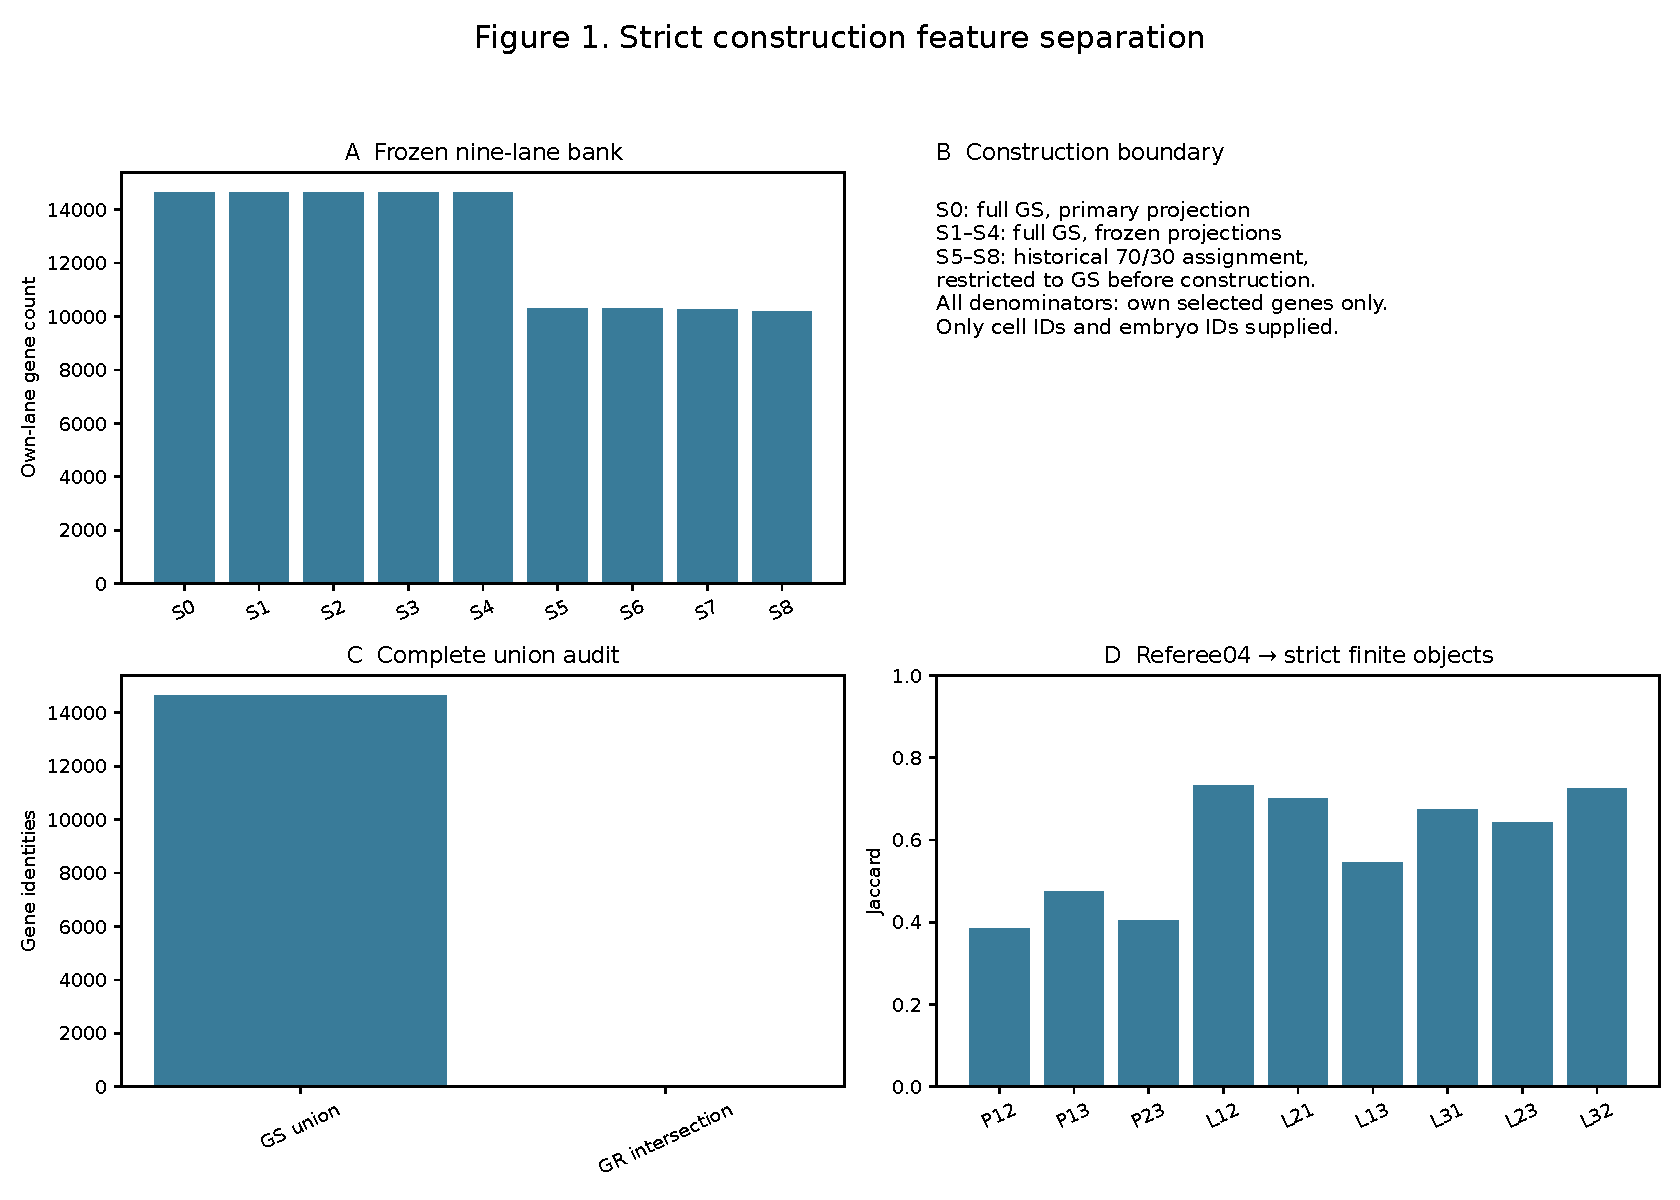
\includegraphics[width=0.98\textwidth]{RMMO_Paper3_Figure1_StrictConstructionConsensus.pdf}
\caption{Strict nine-lane construction and consensus anatomy. (A) Edge counts for all nine pair-specific lane relations. (B) Pair- and lane-specific q50 thresholds. (C) Candidate-edge counts by vote multiplicity; the vertical line marks the seven-of-nine cutoff. (D) Complete feature separation and the exact 7/8/9-vote composition of the strict publication-primary relation.}
\label{fig:construction}
\end{figure}
\FloatBarrier

The consensus vote anatomy is
\[
P12:\ 35+18+6=59,
\]
\[
P13:\ 13+4+0=17,
\]
\[
P23:\ 25+14+5=44,
\]
where the three terms give edges supported by exactly seven, eight, and nine lanes. The strict relations are sparse relative to any individual lane, and their sizes differ substantially across the three embryo pairs. That pair dependence is retained as part of the empirical object and carried into the domain, fiber, and overlap analyses below.

The complete 27 lane/pair thresholds, edge counts, and endpoint counts are available in the Paper 3 public reproducibility companion.



\subsection{q25 fibers reveal a set-valued, directionally asymmetric relation}

The consensus edges define landmark correspondences; the next question is what kind of local mapping they induce around nearby source cells. At q25, every admitted source receives a nonempty target fiber by construction, while fiber multiplicity is an empirical property of the realized relation. The six orientations differ strongly. \(L_{12}\) and \(L_{13}\) are often close to point-like; \(L_{21}\), \(L_{23}\), and \(L_{31}\) carry substantially broader target sets.

\begin{table}[H]
\centering
\scriptsize
\setlength{\tabcolsep}{3.2pt}
\caption{q25 induced-fiber anatomy. ``Multi'' is the fraction of source-domain cells with more than one target.}
\label{tab:fibers}
\begin{tabular}{@{}lrrrrrrrr@{}}
\toprule
Direction & Anchors & Endpoints & Domain & Radius & Median & Mean & Max & Multi\\
\midrule
\(L_{12}\)&50&26&258&0.386974&1&2.217&10&45.7\%\\
\(L_{21}\)&26&50&325&0.463493&5&10.163&36&80.3\%\\
\(L_{13}\)&15&9&258&0.395349&1&1.512&5&36.8\%\\
\(L_{31}\)&9&15&344&0.428213&3&3.933&11&72.4\%\\
\(L_{23}\)&20&36&325&0.466597&3&6.935&25&77.8\%\\
\(L_{32}\)&36&20&344&0.420475&2&2.616&11&63.7\%\\
\bottomrule
\end{tabular}
\end{table}

These multiplicities establish the object type used throughout the remaining analyses. A source cell commonly corresponds to a local set of target cells, making fiber summaries the natural molecular unit for the set-valued geometry. Directional asymmetry is also part of the observed object: median fiber size ranges from one to five, mean size from 1.51 to 10.16, and multi-target occupancy from 36.8\% to 80.3\%.

\subsection{Construction-held-out edges carry molecular agreement beyond the construction panel}

With the finite relation established, the first molecular question is whether its landmark edges remain coherent outside the features used to construct them. The strict geometry is therefore frozen before consensus edges are evaluated in the disjoint molecular panel \(G_R\). Lower \(G_R\) edge distance indicates that the selected landmark pairs share molecular organization that was unavailable to the construction stage.

\begin{table}[H]
\centering
\small
\caption{Construction-held-out landmark-edge agreement. Tails are \(+1\)-corrected empirical tails from 1,024 synchronized reference draws.}
\label{tab:edge_primary}
\begin{tabular}{@{}lrrrrrr@{}}
\toprule
Pair & Observed & Ref. mean & Ref. SD & Reduction & Raw \(p\) & maxT-adjusted \(p\)\\
\midrule
P12&0.3527&0.4241&0.00598&16.83\%&0.000976&0.000976\\
P13&0.3281&0.3968&0.01023&17.31\%&0.000976&0.000976\\
P23&0.3596&0.4292&0.00686&16.21\%&0.000976&0.000976\\
\bottomrule
\end{tabular}
\end{table}

The independently calibrated three-component statistic gives
\[
T_\Sigma=29.1855,\qquad T_{\min}=6.8630,
\]
with both empirical tails equal to \(1/1025\). Here \(T_\Sigma\) summarizes the combined standardized effect across the three embryo pairs, while \(T_{\min}\) asks whether even the weakest of the three standardized effects is unusually strong. All matched-edge strata are feasible without replacement. The selected landmarks therefore retain molecular coherence in \(G_R\). The next analysis asks whether this agreement extends from landmark pairs to the target neighborhoods induced from common source regions.

\subsection{Pair-conditioned target neighborhoods converge in held-out molecular space}

The q25 overlaps identify source cells that participate in two separately pair-derived outgoing systems within the same embryo:
\[
|O_1|=207,\qquad |O_2|=287,\qquad |O_3|=252.
\]
For a cell in \(O_1\), one fiber summarizes its E1--E2 relation and a second fiber summarizes its E1--E3 relation; the same construction applies cyclically in \(O_2\) and \(O_3\). The matched-target analysis asks whether those two pair-conditioned target neighborhoods converge on similar molecular summaries. Its reference preserves target embryo, native fiber cardinality, exact target \(\Czero\) counts, and target anchor-distance-decile counts.

\begin{table}[H]
\centering
\scriptsize
\setlength{\tabcolsep}{3.4pt}
\caption{q25 matched-target molecular coherence. Defect is lower when the two pair-conditioned target summaries agree more closely.}
\label{tab:matched_primary}
\begin{tabular}{@{}llrrrrrr@{}}
\toprule
Panel & Overlap & Observed & Ref. mean & Ref. SD & Reduction & Raw \(p\) & maxT-adjusted \(p\)\\
\midrule
State&O1&0.3234&0.4257&0.00341&24.03\%&0.000976&0.000976\\
State&O2&0.2393&0.2731&0.00179&12.40\%&0.000976&0.000976\\
State&O3&0.2831&0.3463&0.00238&18.23\%&0.000976&0.000976\\
\(G_R\)&O1&0.2581&0.3448&0.00277&25.15\%&0.000976&0.000976\\
\(G_R\)&O2&0.1942&0.2089&0.00138&7.03\%&0.000976&0.000976\\
\(G_R\)&O3&0.2315&0.2719&0.00191&14.88\%&0.000976&0.000976\\
\bottomrule
\end{tabular}
\end{table}

For state defect,
\[
T_\Sigma=74.9651,\qquad T_{\min}=17.3693,
\]
and for \(G_R\) defect,
\[
T_\Sigma=65.8281,\qquad T_{\min}=10.5967.
\]
All four aggregate/minimum tails equal \(1/1025\). The two separately pair-derived views of a common source region therefore converge on held-out molecular summaries more closely than matched target sampling predicts. O2 carries the same direction with a smaller magnitude than O1/O3. The next test fixes endpoint participation and multiplicity to isolate information carried by the observed incidence pattern.

\subsection{Observed connectivity retains source information after fixing endpoints and degrees}

The preceding analyses establish molecular coherence for selected endpoints and for the target neighborhoods induced from common source regions. To localize information to the wiring pattern itself, the source-fidelity reference fixes the exact endpoint populations, exact source degrees, exact target degrees, and graph simplicity, then randomizes which endpoints are connected. Each accepted graph is converted back into induced fibers before target means and source errors are recomputed on the same prespecified overlap cells.

\begin{table}[H]
\centering
\scriptsize
\setlength{\tabcolsep}{3.4pt}
\caption{q25 degree-controlled source fidelity. Lower source error indicates that the induced target fibers preserve more information about the source cell.}
\label{tab:fidelity_primary}
\begin{tabular}{@{}llrrrrrr@{}}
\toprule
Panel & Overlap & Observed & Ref. mean & Ref. SD & Reduction & Raw \(p\) & maxT-adjusted \(p\)\\
\midrule
State&O1&0.3969&0.4260&0.00830&6.83\%&0.000976&0.000976\\
State&O2&0.4230&0.4624&0.00488&8.53\%&0.000976&0.000976\\
State&O3&0.3899&0.4235&0.00748&7.93\%&0.000976&0.000976\\
\(G_R\)&O1&0.3361&0.3429&0.00399&1.99\%&0.0371&0.122927\\
\(G_R\)&O2&0.3547&0.3668&0.00212&3.31\%&0.000976&0.000976\\
\(G_R\)&O3&0.3293&0.3425&0.00322&3.83\%&0.000976&0.000976\\
\bottomrule
\end{tabular}
\end{table}

The state source-error family gives
\[
T_\Sigma=16.0733,\qquad T_{\min}=3.5457,
\]
with both tails equal to \(1/1025\). The held-out source-error family gives
\[
T_\Sigma=11.7093,\qquad T_{\min}=1.6772,
\]
again with both tails equal to \(1/1025\). O1 contributes a positive held-out reduction with calibrated maxT \(p=0.122927\); O2 and O3 retain individual adjusted support. The 1.99--3.83\% held-out reductions are smaller than the matched-target coherence effects because this reference preserves substantially more of the observed relation. Their authority is correspondingly specific: within the declared fixed-endpoint, fixed-degree law, the observed pairing pattern retains source-specific molecular information.

\(T_{\min}\) and component maxT answer different questions. maxT evaluates each named component against the draw-wise maximum across the three components, while \(T_{\min}\) evaluates the weakest observed standardized component against the corresponding synchronized reference distribution. The synchronized three-component result and the individual maxT results therefore support different levels of interpretation.

\begin{figure}[H]
\centering
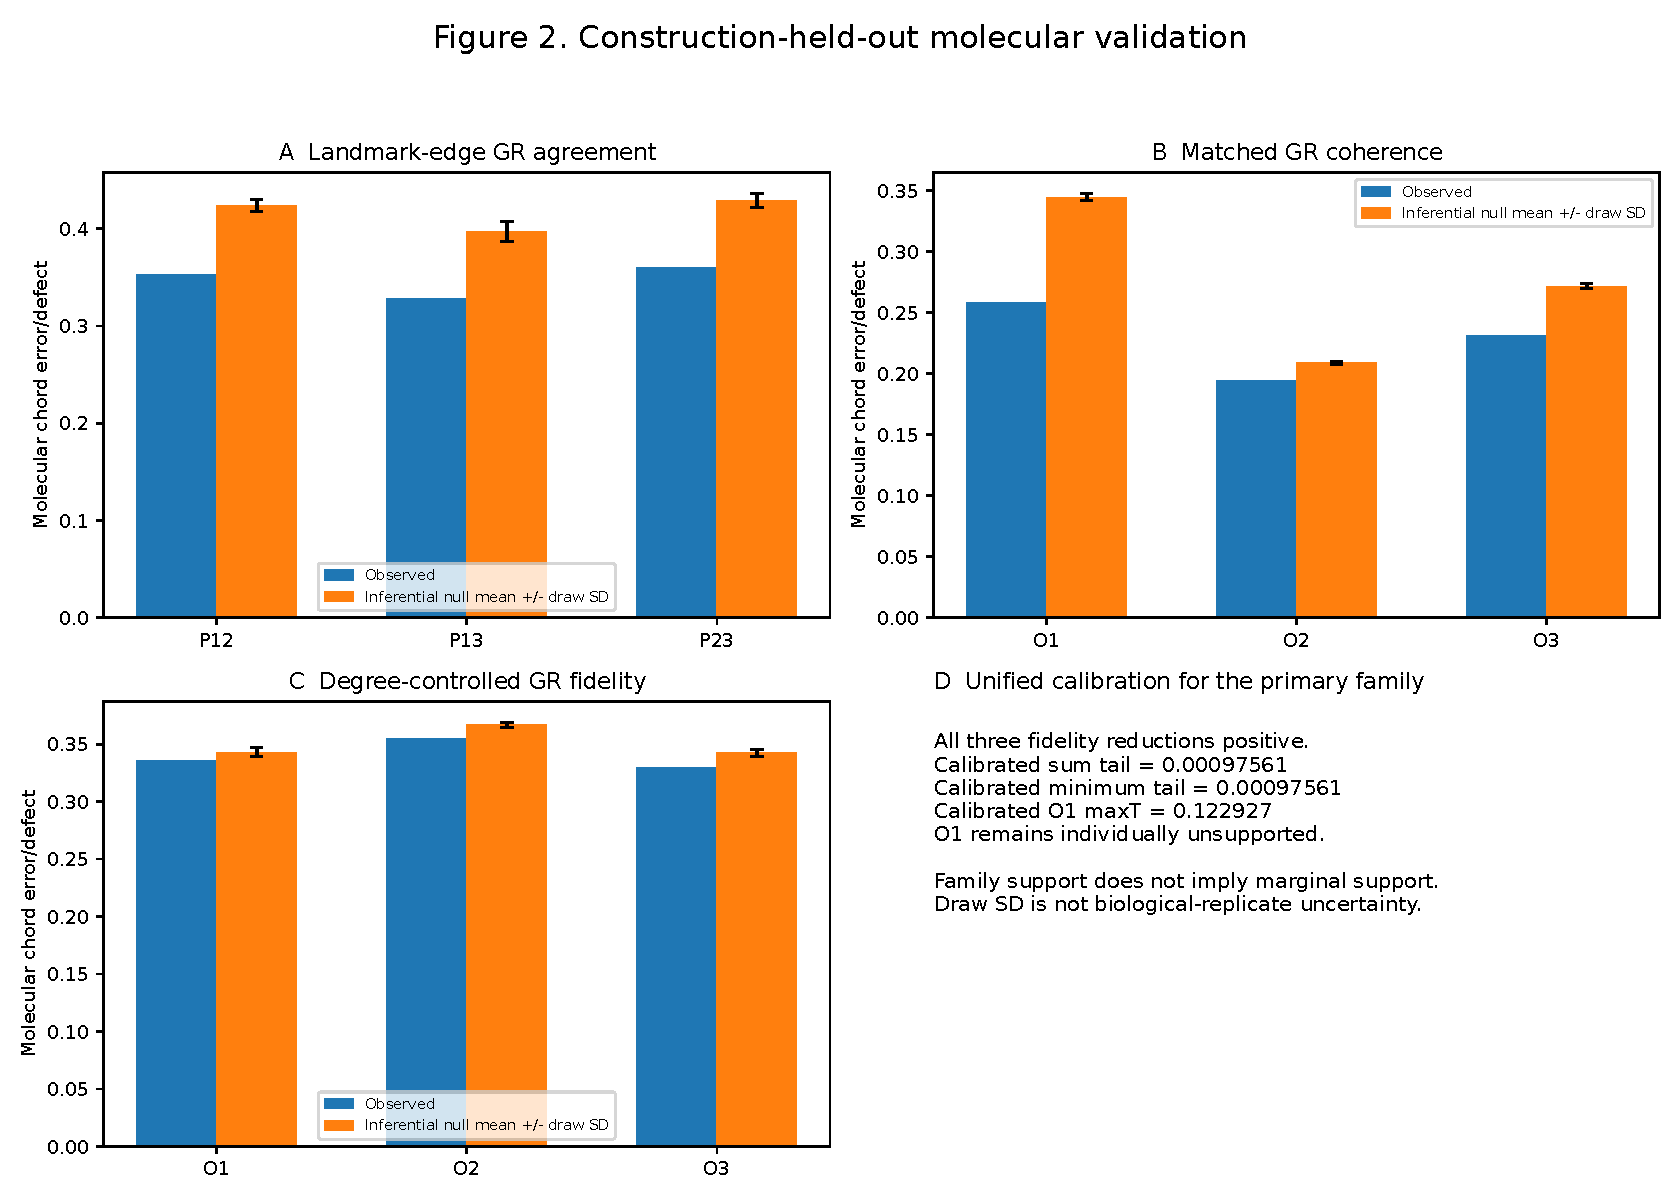
\includegraphics[width=0.98\textwidth]{RMMO_Paper3_Figure2_PrimaryMolecularResults.pdf}
\caption{Primary construction-held-out molecular results. (A) Strict consensus edges show lower \(G_R\) distance than matched cross-pair references. (B) q25 matched-target \(G_R\) coherence. (C) Degree-controlled \(G_R\) source fidelity. (D) O1 has a positive reduction with calibrated maxT \(p=0.122927\); O2/O3 retain individual adjusted support.}
\label{fig:molecular}
\end{figure}
\FloatBarrier

\subsection{Pair-derived source domains converge beyond the spatial reference}

The molecular analyses above are defined on \(O_1,O_2,O_3\), so their spatial origin is itself a biological question. Each overlap is the intersection of two pair-derived source domains inside one embryo. The spatial reference asks whether these separately pair-derived systems concentrate on the same source regions more strongly than expected after matching coarse state, local density, radial position, and local-neighbor spacing. The strict q25 intersections exceed this reference in all three embryos.

\begin{table}[H]
\centering
\small
\caption{q25 spatial source-overlap reference. Enrichment is relative to the matched spatial reference mean.}
\label{tab:s1_primary}
\begin{tabular}{@{}lrrrrrr@{}}
\toprule
Overlap & Observed & Ref. mean & Ref. SD & Enrichment & Raw \(p\) & maxT-adjusted \(p\)\\
\midrule
O1&207&168.54&8.07&22.82\%&0.000976&0.000976\\
O2&287&222.12&11.35&29.21\%&0.000976&0.000976\\
O3&252&209.31&10.81&20.40\%&0.000976&0.000976\\
\bottomrule
\end{tabular}
\end{table}

The synchronized three-component statistic is
\[
T_\Sigma=14.4075,\qquad T_{\min}=3.8952,
\]
with both tails equal to \(1/1025\). The spatial matching reproduces every declared stratum count exactly across all 1,024 draws. The overlap result therefore places the molecular coherence analyses in shared source regions whose concentration exceeds the matched spatial reference.

\subsection{Developmental annotations place the relational geometry in context}

With spatial convergence established, source annotations provide developmental context for the regions participating in the relational object. The strict P12 relation is mesoderm-rich, with mesoderm contributing 57.9\% of pooled landmark endpoints and nascent mesoderm the largest cell type. P13 is more mixed: mesoderm contributes 45.8\%, while rostral ectoderm is the largest single cell type. P23 is strongly mesodermal at 75.0\%, with extraembryonic mesoderm the largest cell type.

The q25 overlaps are similarly heterogeneous. O1 is 64.7\% mesoderm; O2 and O3 are broader, with mesoderm fractions 42.9\% and 40.9\%. These annotations are loaded after geometry construction, so their role here is to locate the inferred source regions within familiar developmental compartments while leaving the construction itself annotation-free.

\begin{figure}[H]
\centering
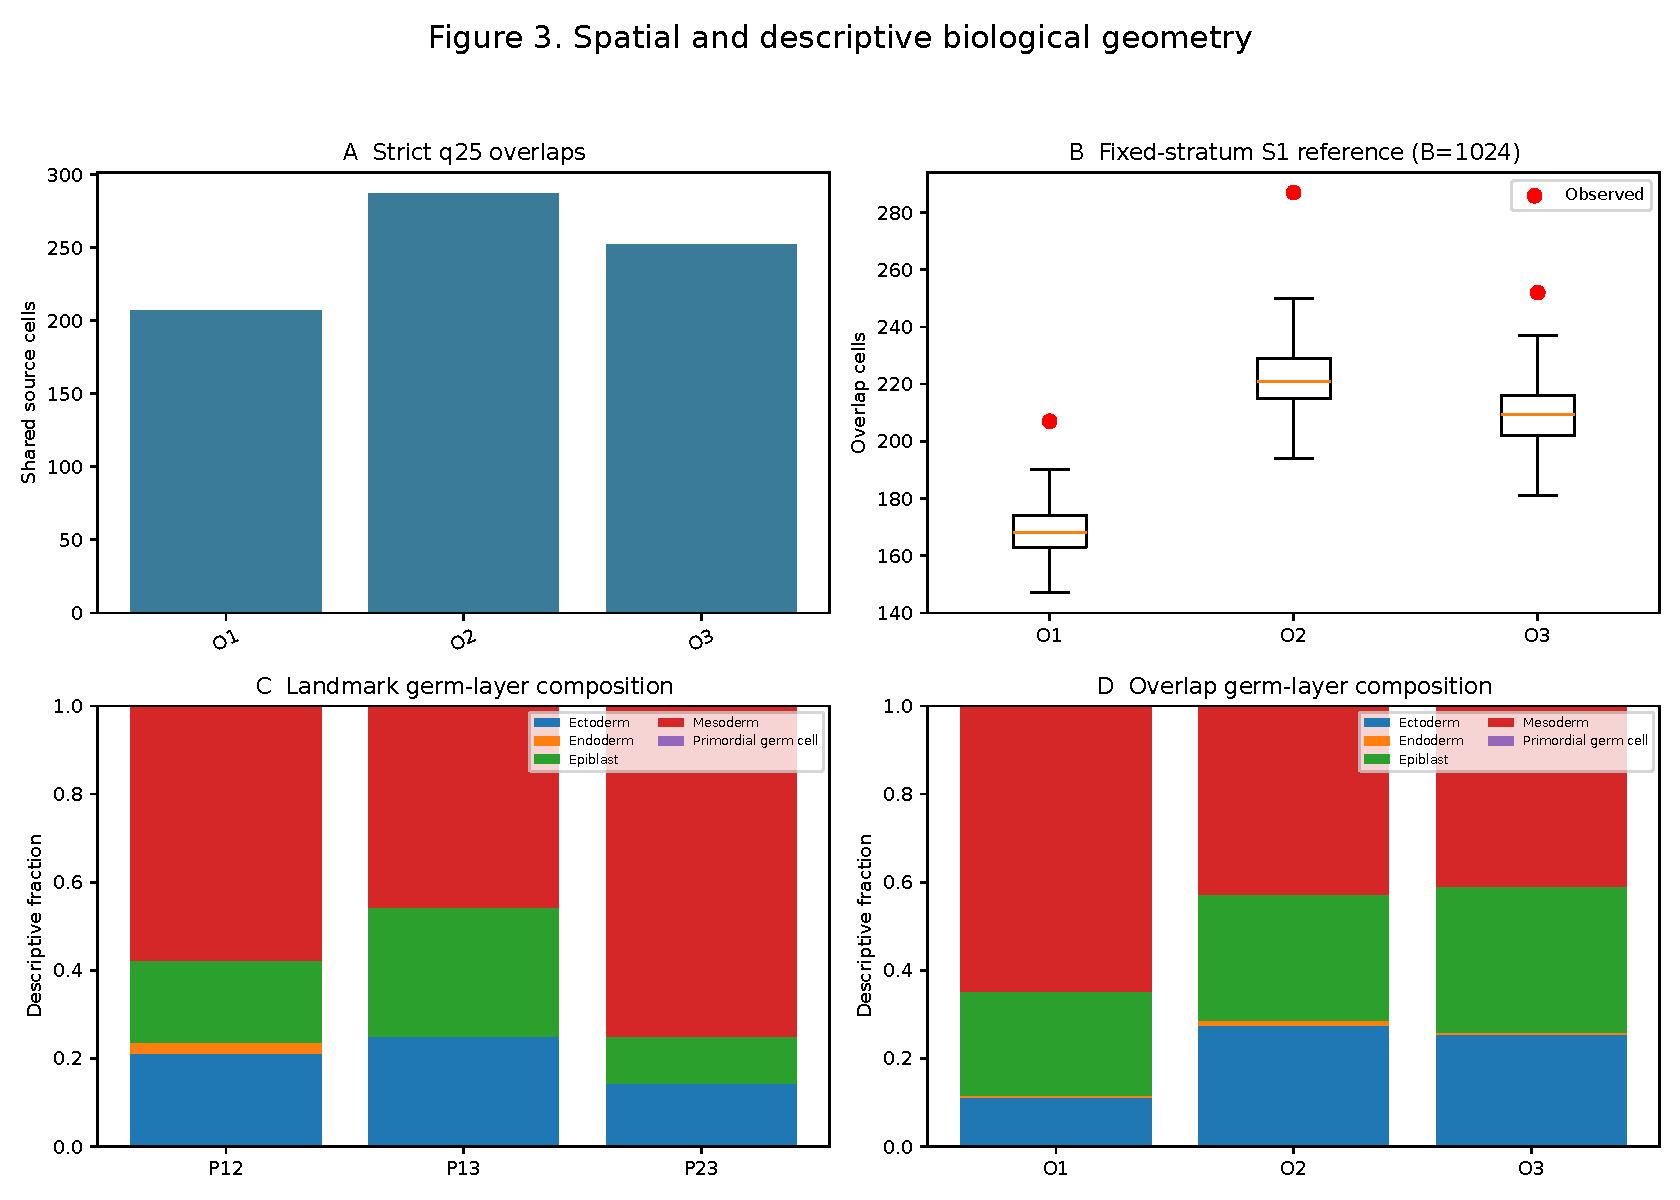
\includegraphics[width=0.98\textwidth]{RMMO_Paper3_Figure3_FiberSpatialBiologicalGeometry.pdf}
\caption{Fiber, spatial, and descriptive biological geometry. (A) Mean q25 target-fiber size across all six orientations. (B) Multi-target fractions. (C) Observed source-domain overlaps versus matched spatial-reference means and SDs. (D) Descriptive mesoderm fractions for landmark and overlap objects.}
\label{fig:fiberspatial}
\end{figure}
\FloatBarrier


\subsection{Pair-conditioned fibers differ from conventional nearest-neighbor neighborhoods}

The pair-conditioned fibers can now be situated against familiar neighborhood constructions. Matched-size kNN asks how well ordinary nearest neighbors perform when target-set size is held equal to the observed fiber. Native MNN \(k=5\) adds reciprocal-neighbor structure and retains approximately 74--78\% of overlap cells. The multiplicity-matched MNN comparison further aligns target multiplicity, with eligible fractions of 46.4\%, 13.6\%, and 12.3\% for O1--O3.

State-space source errors favor the nearest-neighbor baselines. In \(G_R\), matched-size kNN is mixed:
\[
-0.0182,\quad+0.00182,\quad-0.00602
\]
for native-minus-baseline error in O1--O3. Native MNN favors pair-conditioned fibers in all three held-out comparisons:
\[
-0.00307,\quad-0.01743,\quad-0.02029,
\]
and multiplicity-matched MNN likewise:
\[
-0.03194,\quad-0.01103,\quad-0.01988.
\]
These comparisons are descriptive and restricted to their declared common-support cells. They separate preservation of the construction coordinate from preservation of held-out molecular content.

\begin{figure}[H]
\centering
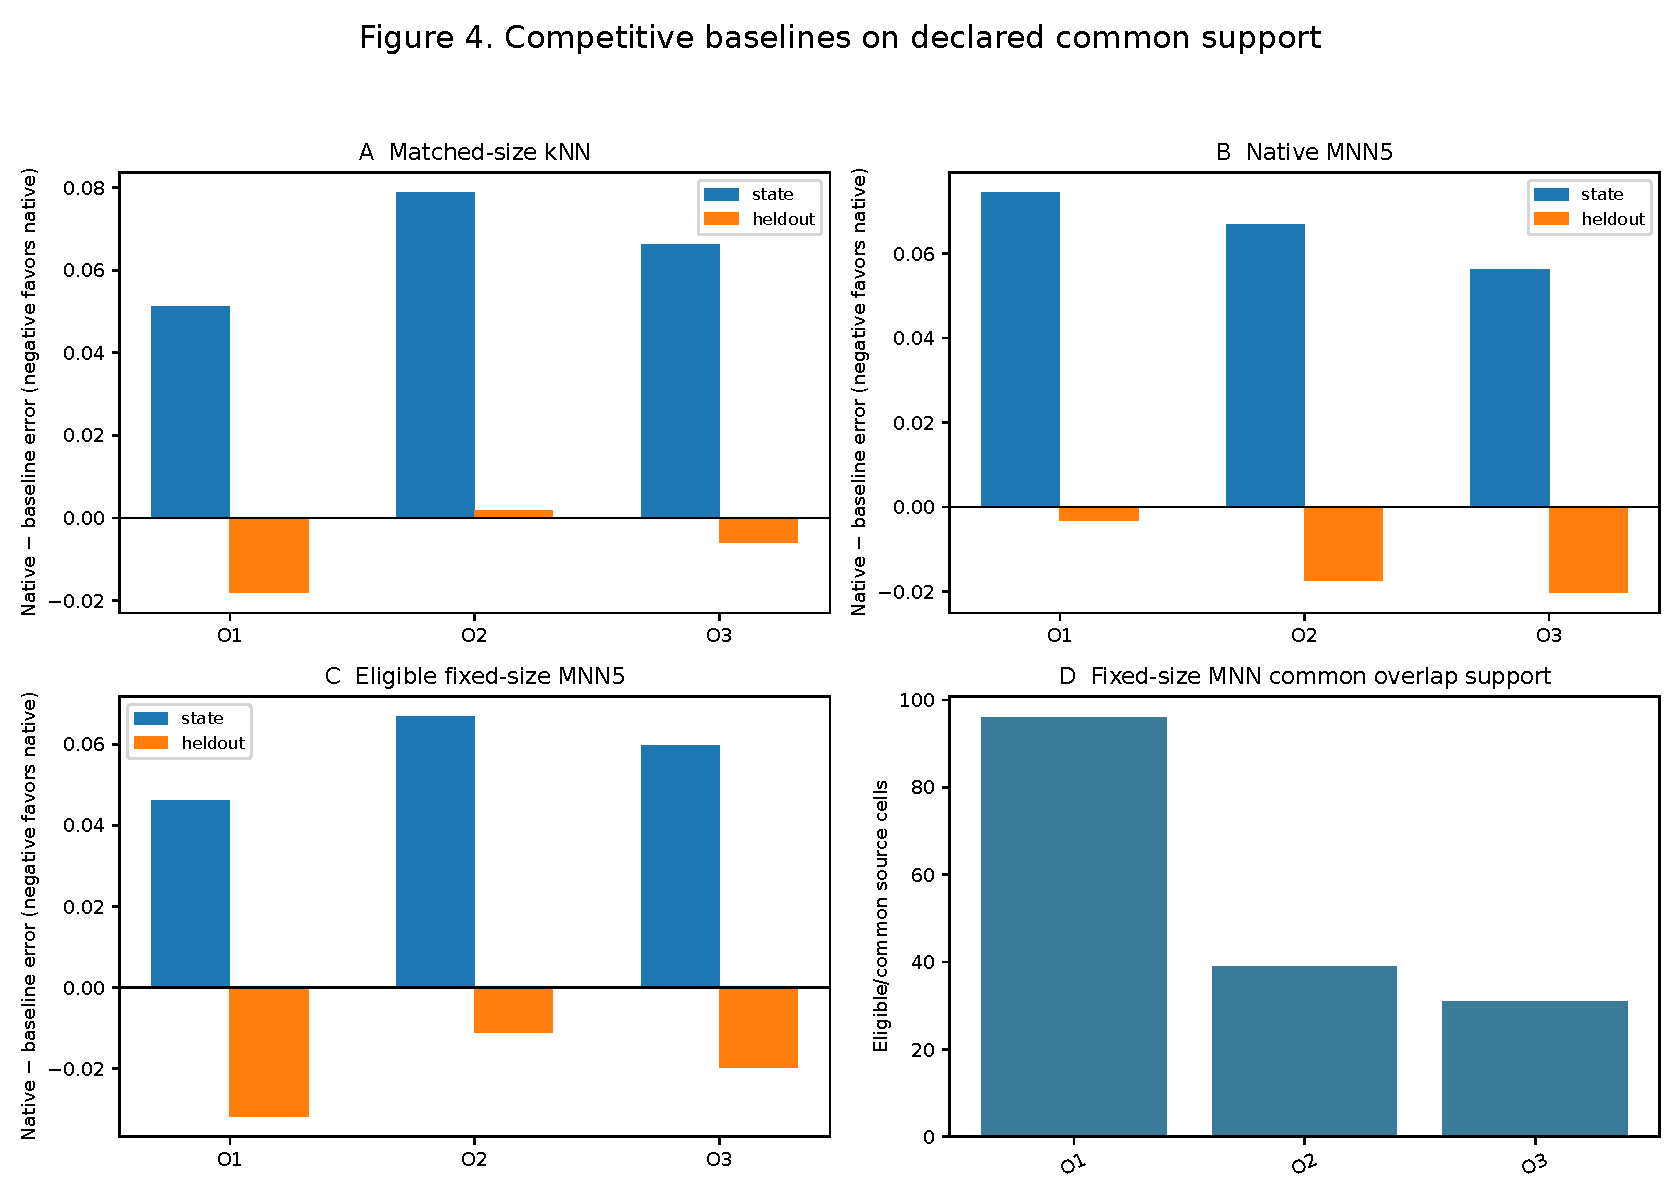
\includegraphics[width=0.98\textwidth]{RMMO_Paper3_Figure4_CompetitiveBaselines.pdf}
\caption{Competitive baseline errors and support. (A) Retained overlap support for matched-size kNN, native MNN5, and multiplicity-matched MNN. (B--D) Pair-conditioned minus comparator source error in state and \(G_R\) coordinates. State-space differences favor the nearest-neighbor comparators; the held-out comparisons show lower pair-conditioned error on most declared common-support sets.}
\label{fig:baselines}
\end{figure}
\FloatBarrier

\subsection{Relational effect direction persists as finite realization changes}

We asked two separate robustness questions. First, how much does stricter feature separation change the finite consensus relation? Second, when the molecular representation is changed from signed-hash coordinates to PCA, does the held-out molecular effect retain its direction? The construction comparison uses the preceding isolated historical-lane consensus and the strict \(G_S\)-only seven-of-nine consensus. The representation comparison uses like-for-like single-representation q50 relations from hash \(\ell_0\), PCA32, and PCA64; the strict consensus remains the publication-primary result.

\begin{table}[H]
\centering
\footnotesize
\setlength{\tabcolsep}{4pt}
\caption{Construction sensitivity only: preceding isolated historical-lane consensus (56/11/36 edges) versus strict consensus (59/17/44). Pair triplets are P12/P13/P23; overlap triplets are O1/O2/O3.}
\label{tab:construction_identity}
\begin{tabular}{@{}lc@{}}
\toprule
Object & Exact-set Jaccard\\
\midrule
Edges & 0.386/0.474/0.404\\
Source endpoints & 0.453/0.562/0.400\\
Target endpoints & 0.429/0.455/0.476\\
q25 overlaps & 0.561/0.682/0.785\\
Six q25 domains & 0.545--0.732\\
\bottomrule
\end{tabular}
\end{table}

Representation-family sensitivity uses the single \(\ell_0\) hash lane as its reference object, with the 59/17/44 strict consensus retained as the publication-primary construction. The \(\ell_0\) q50 edge counts are 4798/4355/4959 for P12/P13/P23. PCA32 uses 4322/3023/6416 and PCA64 uses 4910/3405/7230. PCA32 and PCA64 retain 23.62\% and 26.18\% of centered expression energy, respectively.

\begin{table}[H]
\centering
\footnotesize
\setlength{\tabcolsep}{4pt}
\caption{Like-for-like single-lane representation sensitivity. Jaccards compare each PCA row with the hash \(\ell_0\) relation. Edge triplets are P12/P13/P23; overlap and \(G_R\)-reduction triplets are O1/O2/O3. Domain range spans the six q25 orientations.}
\label{tab:representation}
\begin{tabular}{@{}lcccc@{}}
\toprule
Lane & Edge Jaccard & Domain Jaccard range & Overlap Jaccard & \(G_R\) reduction (\%)\\
\midrule
Hash \(\ell_0\) & 1/1/1 & 1--1 & 1/1/1 & 5.34/5.39/4.84\\
PCA32 & 0.025/0.021/0.029 & 0.215--0.261 & 0.188/0.169/0.143 & 6.08/4.67/3.35\\
PCA64 & 0.031/0.026/0.033 & 0.206--0.252 & 0.186/0.188/0.165 & 6.58/4.63/4.32\\
\bottomrule
\end{tabular}
\end{table}

Every single-lane \(G_R\) matched-defect reduction is positive, while hash-\(\ell_0\)/PCA edge Jaccards are only 0.021--0.033, q25 domain Jaccards are approximately 0.206--0.261, and overlap-cell Jaccards are approximately 0.143--0.188. Across the tested representations, the molecular relational effect retains its direction while edge, domain, and overlap membership change substantially. This sensitivity is measured within the same three embryos.

The publication-primary strict consensus remains the main inferential object, with matched \(G_R\) q25 reductions of 25.15\%, 7.03\%, and 14.88\%. The single-lane hash/PCA controls measure how effect direction behaves as the representation changes, while the consensus result carries the primary molecular estimate.

\begin{figure}[H]
\centering
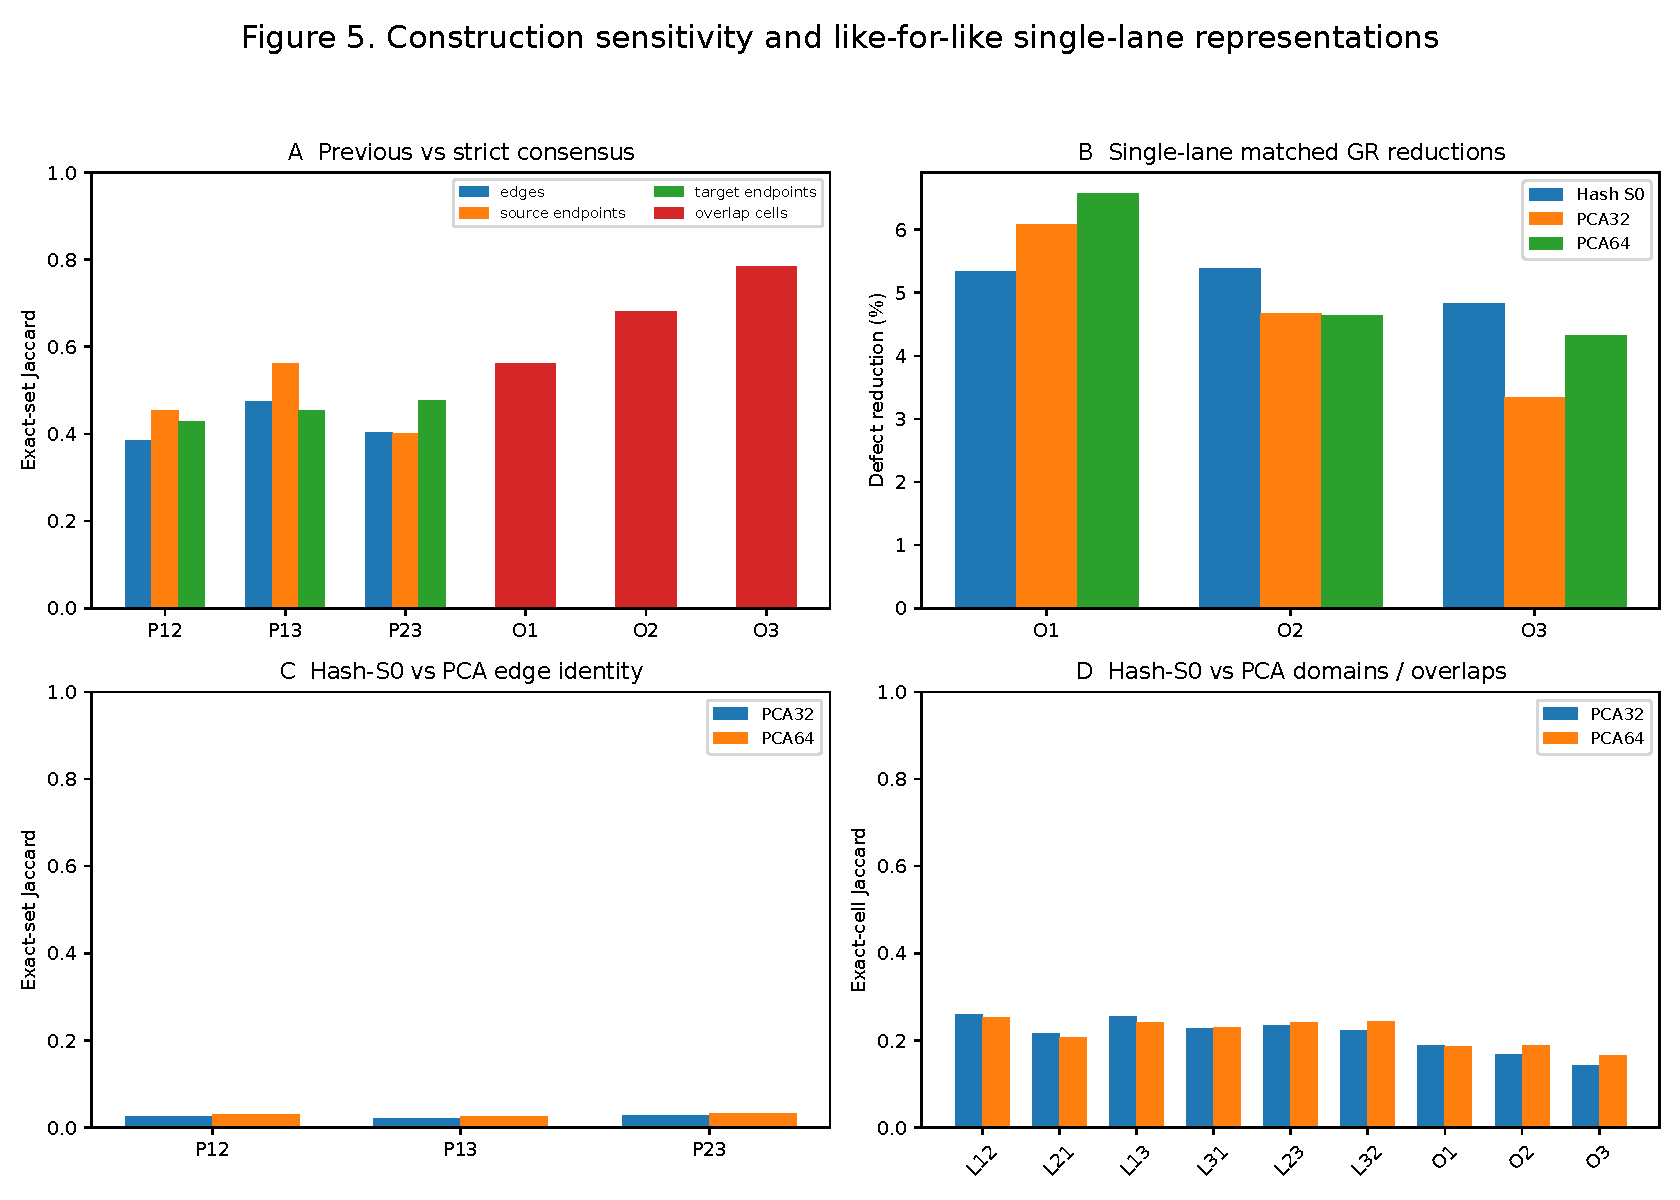
\includegraphics[width=0.98\textwidth]{RMMO_Paper3_Figure5_ConstructionRepresentationSensitivity.pdf}
\caption{Construction and representation sensitivity. (A) Exact-set Jaccards for the preceding versus strict consensus construction. (B) Like-for-like single-lane hash \(\ell_0\), PCA32, and PCA64 \(G_R\) matched-defect reductions. (C) Hash \(\ell_0\) versus PCA edge Jaccards. (D) All six q25 domain and three overlap-cell Jaccards. The molecular effect remains positive across tested representations while finite membership changes substantially; strict-consensus effects are reported separately.}
\label{fig:pca}
\end{figure}
\FloatBarrier

\subsection{The principal directions persist across prespecified domain scales}

Representation perturbations change the molecular coordinate used to realize a relation; domain-scale perturbations change how far that relation is extended around its source landmarks. The q50 lane scale, seven-of-nine consensus threshold, and q25 primary domain scale were specified before molecular outcome evaluation, with q10 and q50 designated in advance as narrower and broader domain sensitivities.

\begin{table}[H]
\centering
\footnotesize
\setlength{\tabcolsep}{4pt}
\caption{Prespecified strict-consensus domain-scale sensitivity. Reductions are percentages; maxT and synchronized three-component tails use independently fixed calibration constants with the original inferential draws supplying ranks. q25 remains the publication-primary domain scale.}
\label{tab:scales}
\begin{tabular}{@{}llrrrrrr@{}}
\toprule
Test & Scale & O1 & O2 & O3 & \(p_\Sigma\) & \(p_{\min}\) & O1 maxT-adjusted \(p\)\\
\midrule
Matched \(G_R\) defect & q10 & 25.07 & 7.73 & 15.09 & 0.000976 & 0.000976 & 0.000976\\
Matched \(G_R\) defect & q25 & 25.15 & 7.03 & 14.88 & 0.000976 & 0.000976 & 0.000976\\
Matched \(G_R\) defect & q50 & 23.80 & 5.21 & 13.60 & 0.000976 & 0.000976 & 0.000976\\
Degree \(G_R\) source error & q10 & 4.48 & 4.71 & 4.14 & 0.000976 & 0.000976 & 0.060488\\
Degree \(G_R\) source error & q25 & 1.99 & 3.31 & 3.83 & 0.000976 & 0.000976 & 0.122927\\
Degree \(G_R\) source error & q50 & 1.23 & 2.23 & 2.82 & 0.000976 & 0.001951 & 0.139512\\
\bottomrule
\end{tabular}
\end{table}

All source-fidelity component directions remain positive. O1 has calibrated maxT tails of 0.060488, 0.122927, and 0.139512 at q10, q25, and q50, respectively, while the synchronized three-component test remains supported at each scale. The q50 weakest-component tail is \(2/1025\). The principal molecular directions therefore persist across the prespecified domain scales, with degree-controlled magnitude varying more strongly than matched-target coherence. Independent calibration of all standardized scores leaves every reported support decision unchanged (Methods; Paper 3 public reproducibility companion).


\subsection{\(R0\)--\(R3\) reveal how lower-order structure progressively explains the effect}

The established relation carries spatial and molecular organization. The \(R0\)--\(R3\) sequence asks how much of that organization can be reproduced as progressively richer lower-order structure is restored.

The retained-structure references are:
\begin{itemize}[leftmargin=2em]
\item \(R0\) (\emph{size only}): source domains and target-set sizes;
\item \(R1\) (\emph{+ coarse state}): \(R0\) plus sourcewise target \(C_0\) histograms;
\item \(R2\) (\emph{+ anchor proximity}): \(R1\) plus target anchor-distance deciles;
\item \(R3\) (\emph{+ endpoint support}): \(R2\) plus restriction to observed target endpoint populations.
\end{itemize}


The effect surface is more informative than the common tail floor. For O1 state defect, the null mean moves:
\[
0.5246\rightarrow0.5106\rightarrow0.4257\rightarrow0.3740
\]
from \(R0\) to \(R3\), toward the observed
\[
0.3234.
\]
For O1 \(G_R\) source error:
\[
0.3958\rightarrow0.3853\rightarrow0.3686\rightarrow0.3550,
\]
toward observed
\[
0.3361.
\]

The largest shift occurs for O1 state defect:
\[
0.52462\rightarrow0.37399,
\]
a change of approximately \(0.15063\). As progressively richer structure is retained, the reference distributions move toward the observed data, showing how target-set size, coarse composition, anchor-distance organization, and endpoint support account for part of the measured effect. A residual separation remains after \(R3\). This conclusion applies to the four tested retained-structure references; other mechanisms remain possible.

\subsection{Exact global compatibility remains absent}

The preceding analyses establish coherent pair-local organization. The final Results question asks whether the three pairwise systems also satisfy the stronger exact compatibility conditions required for a single globally consistent correspondence. For induced q25 fiber relations
\[
C_{ij}
=
\{(x,y):x\in U_i^{ij}(0.25),\ y\in F_{ij}^{0.25}(x)\},
\]
ordinary composition is tested directly.

The route \(1\to2\to3\) contains:
\[
329\ \text{direct pairs},\qquad
4161\ \text{composed pairs},\qquad
250\ \text{common},
\]
leaving 79 direct-only and 3911 composed-only pairs.

For \(1\to3\to2\):
\[
517,\quad1677,\quad371,
\]
leaving 146 direct-only and 1306 composed-only pairs.

For \(2\to1\to3\):
\[
2105,\quad862,\quad321,
\]
leaving 1784 direct-only and 541 composed-only pairs.

No route satisfies exact equality.

The historical common-refinement diagnostic is also shown directly. For source cell \(x\in O_i^{jk}\), let
\[
B_x=
(F_{ij}^{0.25}(x)\times F_{ik}^{0.25}(x))
\cap L_{jk}.
\]
The implemented historical criterion calls \(x\) refinable when
\[
|B_x|>0.
\]
The implemented bridge criterion is existential: a source cell passes when at least one target pair is linked by the third relation. It places no universal coverage requirement on all target partners. Under this criterion:
\[
O_1:\ 165/207\ \text{pass},
\]
\[
O_2:\ 168/287,
\]
\[
O_3:\ 186/252.
\]
No overlap is completely refinable. Together with the direct/composed mismatches, these counts place the measured organization at a local, pair-conditioned level under the tested compatibility criteria.

\begin{figure}[H]
\centering
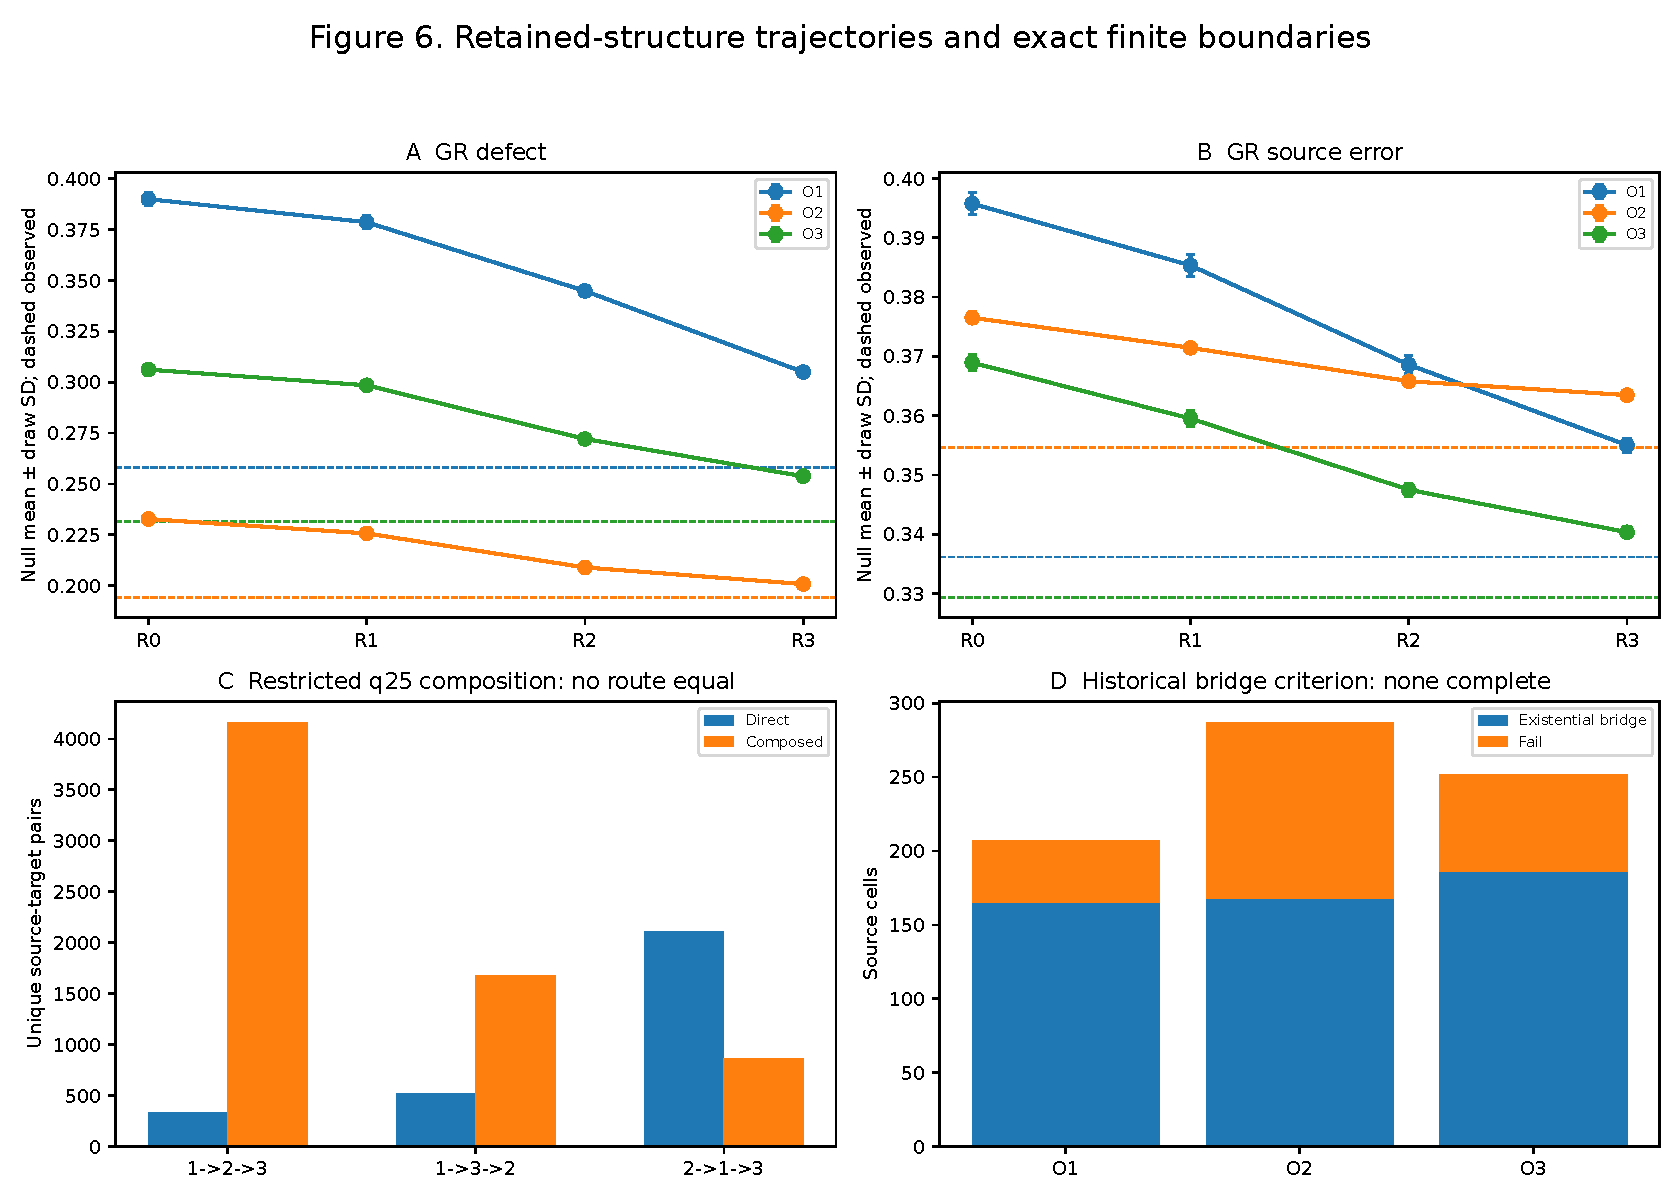
\includegraphics[width=0.98\textwidth]{RMMO_Paper3_Figure6_RetentionGlobalBoundary.pdf}
\caption{Retained-structure effects and exact finite boundaries. (A,B) Selected \(G_R\) and state reference means move toward observation from \(R0\) (size only) to \(R3\) (+ endpoint support). (C) Direct and composed restricted q25 relation counts show routewise inequality. (D) The historical existential bridge criterion fails on nonzero subsets of every overlap, so complete common refinement is absent.}
\label{fig:global}
\end{figure}
\FloatBarrier

\FloatBarrier
\section{Discussion}

\subsection{Local relational organization as a developmental object}

The E7.5 carrier supports a pair-conditioned relational object with a clear biological interpretation. Its target fibers are genuinely set-valued and strongly direction-dependent, its separately pair-derived source domains converge on shared regions within each embryo, and those shared regions map to target neighborhoods with coherent molecular summaries in \(G_R\). The relation therefore organizes correspondence at the level of local neighborhoods, with a single source cell often linked to several plausible partners in another embryo.

The molecular evidence becomes progressively more specific across the primary tests. Landmark edges are coherent in features excluded from construction. Pair-conditioned target sets originating from the same source region converge in held-out molecular space. After endpoint populations and degree sequences are fixed, the observed pairing pattern still carries a smaller but reproducible amount of source-specific \(G_R\) information. This last result localizes part of the molecular preservation to connectivity itself.

Developmental annotations place these relations in recognizable embryonic contexts. P12 and P23 are enriched for mesodermal endpoints, while P13 is more compositionally mixed, and the three overlap regions differ in their germ-layer composition. These annotations were introduced after relation construction, so they provide biological context for an independently defined geometry. Taken together, the results support local cross-embryo organization through neighborhoods and incidence patterns at a stage where a unique cell-to-cell correspondence is not required by the data.

\subsection{Stable molecular effects across changing realizations}

The competitive and representation analyses show that correspondence depends on the property being preserved. Conventional kNN and MNN neighborhoods perform strongly in the state coordinate used to define proximity, while pair-conditioned fibers retain favorable \(G_R\) source-error behavior on several declared common-support comparisons. These observations separate geometric proximity in the construction space from preservation of molecular information in a disjoint feature panel.

The same distinction appears more sharply under representation perturbation. Hash-\(\ell_0\), PCA32, and PCA64 generate substantially different edge sets, source domains, and overlap memberships, yet all three retain positive matched \(G_R\) effect directions. The prespecified q10/q25/q50 analysis gives a complementary result across neighborhood scale: matched-target coherence remains directionally stable, while degree-controlled source fidelity varies more in magnitude and keeps the same three-component direction.

This combination suggests a useful developmental interpretation. Reproducible cross-embryo organization can reside in a relational property even when the particular cells and edges that realize it depend on representation or neighborhood scale. The current data establish that statement within the same three E7.5 embryos. They provide a defined local object and a measured stability profile that can be carried forward into independent cross-horizon reconstruction.

\subsection{Lower-order explanation and the local-to-global boundary}

The \(R0\)--\(R3\) analysis shows how progressively richer retained structure moves the reference distributions toward the observed statistics. Target-set size, coarse molecular composition, anchor-distance organization, and endpoint support each account for part of the measured discrepancy. The remaining separation after \(R3\) therefore belongs to the residual organization left after those specific ingredients have been preserved.

The pairwise systems also have a direct structural boundary. Routewise composition produces relations that differ substantially from the corresponding direct relations, and the historical existential bridge condition fails for nonzero subsets of all three source overlaps. The supported organization therefore remains pair-local under the tested exact compatibility criteria. A single exact cross-embryo equivalence is not required to account for the molecular and spatial effects measured here.

For developmental biology, this distinction matters because embryo-to-embryo reproducibility can be expressed through overlapping local neighborhoods and their molecular organization. Such reproducibility can coexist with heterogeneous fiber multiplicity, pair asymmetry, changing membership, and incomplete global compatibility. An important next question is whether this form of local organization recurs when later developmental stages are reconstructed separately.

\FloatBarrier
\section{Scope and limitations}

Biological replication is limited to three E7.5 embryos. The inferential hierarchy, representation controls, and reference models were developed and stress-tested on this same carrier, so independent embryos or an external dataset are required for biological confirmation beyond the present system. Cells, edges, representation lanes, and randomization draws improve characterization of the measured carrier while leaving biological \(n=3\).

The \(G_R\) panel is held out from numerical relation construction and remains measured in the same cells and experiment. Its results therefore support feature-held-out molecular evaluation within this carrier. The multiplicity-matched MNN control has restricted support, especially in O2 and O3, and the PCA analyses quantify representation sensitivity within the same embryos.

The \(R0\)--\(R3\) conclusions apply to the four tested retained-structure references. The exact common-refinement analysis uses the implemented existential bridge criterion. The study establishes local pair-conditioned organization within these embryos; causal lineage mechanisms, population-level developmental laws, representation invariance, and a single exact global biological equivalence remain outside the present empirical scope.

\FloatBarrier
\section{Methods}

The q50 lane relation scale, seven-of-nine consensus threshold, and q25 primary domain scale were inherited unchanged from the frozen pre-evaluation analysis plan and were not selected from the present \(G_R\) outcomes. The q10 and q50 domain-scale sensitivities were also frozen before acceptance-stage display analyses.


\subsection{Carrier construction and coarse state}

The source is MELA v1, Zenodo record 10.5281/zenodo.19892785 \cite{Colgan2026}. The deposited E7.5-R1, E7.5-R2, and E7.5-R3 files are denoted E1, E2, and E3 in the manuscript. An embryo carrier \(X_i\) contains transcriptome cell IDs assigned to the source-owned lineage tree and present among its nodes. The exact-ID audit traverses the parent path for each observed cell; no minimum lineage depth or edit threshold is imposed.

Carrier flow is:
\[
E1:\ 1342\rightarrow1032,\qquad
E2:\ 1838\rightarrow1298,\qquad
E3:\ 1468\rightarrow1374.
\]
Every lineage-qualified ID joins the transcriptome table exactly, with zero unmatched cells and zero additional biological filtering after qualification.

The coarse matching state is:
\[
\Czero=
\texttt{germ\_layer|phase|type}.
\]
It is source metadata used for matching and stratification. Its realized categories are shown in Table~\ref{tab:C0}.

\begin{longtable}{@{}lrrrr@{}}
\caption{Realized coarse-state \(C_0\) categories.}
\label{tab:C0}\\
\toprule
Category & E1 & E2 & E3 & Total\\
\midrule
\endfirsthead
\toprule
Category & E1 & E2 & E3 & Total\\
\midrule
\endhead
Ectoderm|G2/M|donor&152&234&278&664\\
Ectoderm|S|donor&63&61&95&219\\
Endoderm|G2/M|donor&30&58&26&114\\
Endoderm|S|donor&9&9&13&31\\
Epiblast|G2/M|donor&183&290&314&787\\
Epiblast|S|donor&83&87&146&316\\
Mesoderm|G0/G1|donor&2&5&0&7\\
Mesoderm|G2/M|donor&445&485&432&1362\\
Mesoderm|S|donor&62&67&68&197\\
Primordial germ cell|G2/M|donor&0&2&2&4\\
Primordial germ cell|S|donor&3&0&0&3\\
\bottomrule
\end{longtable}

\subsection{Prespecified gene partition}

A source gene is eligible when it is detected in at least 1\% of cells in at least two embryos, has positive mean in at least one embryo, has false source \texttt{var/mito} flag, and does not begin with the case-sensitive \texttt{Rpl} or \texttt{Rps} prefix. Of 78,258 source features, 20,999 satisfy these criteria.

Let
\[
H(s)=
\operatorname{uint64}_{\rm BE}
\left(
\operatorname{SHA256}(\operatorname{UTF8}(s))[0{:}8]
\right).
\]
Eligible stable gene ID \(g\) is assigned to \(G_S\) when
\[
H(\texttt{RMMO12\_STATE\_REALIZATION\_V1}|g)\bmod 10<7,
\]
and otherwise to \(G_R\). This yields:
\[
|G_S|=14{,}660,\qquad |G_R|=6{,}339,\qquad G_S\cap G_R=\varnothing.
\]
The partition is inherited unchanged from the predecessor analysis and uses neither annotation nor downstream outcomes.

\subsection{Own-lane normalization and signed-hash projection}

For lane gene set \(G_\ell\), raw count \(c_g(x)\), and cell \(x\),
\[
h_g^\ell(x)=
\log\left(
1+\frac{10^4 c_g(x)}
{\sum_{u\in G_\ell} c_u(x)}
\right).
\]
Zero selected-library rows map to zero.

For projection seed \(s_\ell\),
\[
b_\ell(g)
=
H(s_\ell|\texttt{bucket}|g)\bmod64,
\]
and
\[
\sigma_\ell(g)=
\begin{cases}
+1,&H(s_\ell|\texttt{sign}|g)\bmod2=0,\\
-1,&\text{otherwise}.
\end{cases}
\]
The unnormalized coordinate is:
\[
u_{\ell,r}(x)
=
\sum_{g:b_\ell(g)=r}
\sigma_\ell(g)h_g^\ell(x),
\]
followed by:
\[
Z_\ell(x)=
\frac{u_\ell(x)}{\|u_\ell(x)\|_2}
\]
for nonzero rows.

Lane \(\ell_0\) uses all \(G_S\) genes with the primary projection seed. Lanes \(\ell_1,\ldots,\ell_4\) use all \(G_S\) genes with four prespecified alternate projection seeds. Lanes \(\ell_5,\ldots,\ell_8\) use the primary projection seed and deterministic \(G_S\)-only 70\% subpanels:
\[
g\in G_{\ell}
\iff
H(\texttt{panel-seed}_\ell|g)\bmod10<7.
\]
Their realized sizes are 10,300, 10,307, 10,268, and 10,207 genes.

The evaluation coordinate \(\ZR\) is constructed analogously from \(G_R\) with its own \(G_R\)-only library denominator and prespecified evaluation projection seed. \(G_R\) is unavailable to numerical relation construction.

\subsection{Construction/evaluation firewall}

Stage A receives only:
\begin{itemize}[leftmargin=2em]
\item selected \(G_S\) counts;
\item ordered \(G_S\) gene identities;
\item cell and embryo identities;
\item prespecified seeds/constants.
\end{itemize}
It reads no \(G_R\) counts, \(\ZR\), annotations, lineage/history, or evaluation statistics.

The complete numerical geometry is fixed before Stage B reveals \(\ZR\). As a software-level noninterference audit, 7,944,627 stored \(G_R\) values are deterministically replaced while \(G_S\) bytes are preserved. Re-executing the construction yields byte-identical hashes for all 219 numerical geometry arrays and the compressed geometry container. This verifies computational noninterference and is not biological evidence.

\subsection{State distance, lane thresholds, and consensus edges}

For lane-normalized unit rows,
\[
d_\ell(x,y)
=
\|Z_\ell(x)-Z_\ell(y)\|_2
=
\sqrt{
\max\left(
0,
2-2\langle Z_\ell(x),Z_\ell(y)\rangle
\right)
}.
\]
The primary state distance is \(d_S=d_{\ell_0}\).

For embryo pair \(i,j\),
\[
m_{i\to j}^{\ell}(x)
=
\min_{y\in X_j}d_\ell(x,y),
\]
and the pair-symmetric q50 threshold is:
\[
\epsilon_{ij}^{\ell}
=
Q_{0.5}
\left(
\{m_{i\to j}^{\ell}(x):x\in X_i\}
\uplus
\{m_{j\to i}^{\ell}(y):y\in X_j\}
\right),
\]
using NumPy's linear-interpolated quantile.

The lane edge set is:
\[
L_{ij}^{\ell}
=
\{(x,y)\in X_i\times X_j:
d_\ell(x,y)\le\epsilon_{ij}^{\ell}\}.
\]
All threshold ties are retained. Within-embryo edges are impossible by construction. One shared threshold is used for both directions; the reverse relation is the transpose.

For candidate edge \(e\),
\[
v(e)=
\sum_{\ell=0}^{8}
\mathbf 1[e\in L_{ij}^{\ell}],
\]
and:
\[
L_{ij}
=
\{e:v(e)\ge7\}.
\]

\subsection{Domains, active anchors, fibers, and overlaps}

Let \(A_{ij}\) be the source endpoints of the consensus relation and:
\[
T_{ij}(a)=
\{y:(a,y)\in L_{ij}\}.
\]
Define:
\[
\rho_{ij}(x)=
\min_{a\in A_{ij}}d_S(x,a),
\]
\[
r_{ij}(q)=
Q_q
\left(
\{\rho_{ij}(x):x\in X_i\}
\right),
\]
and:
\[
U_i^{ij}(q)
=
\{x:\rho_{ij}(x)\le r_{ij}(q)\}.
\]
Ties at the radius are retained.

Active source anchors are:
\[
A_{ij}^{q}(x)=
\{a\in A_{ij}:d_S(x,a)\le r_{ij}(q)\}.
\]
The set-valued target fiber is:
\[
F_{ij}^{q}(x)=
\bigcup_{a\in A_{ij}^{q}(x)}
T_{ij}(a),
\]
with duplicate target cells removed.

For outgoing pairs \(i\to j\) and \(i\to k\),
\[
O_i^{jk}(q)
=
U_i^{ij}(q)\cap U_i^{ik}(q).
\]
q25 is primary; q10 and q50 are prespecified sensitivities.

\subsection{State and molecular target summaries}

For \(P\in\{S,R\}\), let:
\[
\bar M_P^{ij}(x)
=
\frac1{|F_{ij}^q(x)|}
\sum_{y\in F_{ij}^q(x)}
Z_P(y).
\]
For state coordinates, target means are re-unit-normalized:
\[
M_S^{ij}(x)=
\frac{\bar M_S^{ij}(x)}
{\|\bar M_S^{ij}(x)\|_2}.
\]
For \(G_R\),
\[
M_R^{ij}(x)=\bar M_R^{ij}(x).
\]

For \(O=O_i^{jk}(q)\), overlap defect is:
\[
D_P(O)=
\frac1{|O|}
\sum_{x\in O}
\|
M_P^{ij}(x)-M_P^{ik}(x)
\|_2,
\]
and source error is:
\[
E_P(O)=
\frac1{2|O|}
\sum_{x\in O}
\left(
\|Z_P(x)-M_P^{ij}(x)\|_2+
\|Z_P(x)-M_P^{ik}(x)\|_2
\right).
\]

\subsection{Fixed-stratum spatial reference}

For each source cell, density is defined as the 10th nearest within-embryo \(d_S\) distance, excluding self. Density strata are quartiles over the complete source embryo.

Local-NN distance is the nearest within-embryo \(d_S\) distance, excluding self. Local-NN strata are deciles over the complete source embryo.

For orientation \(i\to j\), radial distance is:
\[
r^{\rm rad}_{ij}(x)
=
\|
Z_S(x)-\overline Z_S(A_{ij})
\|_2,
\]
where \(\overline Z_S(A_{ij})\) is the arithmetic mean of observed source-anchor coordinates and is not renormalized. Radial strata are orientation-specific deciles over the source embryo.

The complete spatial-matching stratum is:
\[
(\Czero,\text{density quartile},\text{radial decile},\text{local-NN decile}).
\]
Quantile cutpoints use linear interpolation; `searchsorted(side='right')` sends ties to the higher bin.

Each draw independently samples the exact observed number of landmarks without replacement from every fixed stratum and then refits the q25 source-domain radius. Across all 1,024 draws, maximum stratum imbalance is zero.

\subsection{Matched-target and matched-edge references}

For target cell \(y\), define target anchor distance:
\[
a_{ij}(y)
=
\min_{b\in \mathrm{target}(L_{ij})}
d_S(y,b).
\]
Its deciles are computed over the entire target embryo with right-bin tie handling.

The matched-target law preserves, source by source:
\begin{itemize}[leftmargin=2em]
\item target embryo;
\item fiber cardinality;
\item exact target \(\Czero\) histogram;
\item exact target-anchor-distance-decile histogram.
\end{itemize}
Sampling is uniform without replacement inside each complete-target-embryo stratum. There are zero impossible strata, zero fallbacks, and zero replacement events.

The realized request diagnostics are:

\begin{table}[htbp]
\centering
\small
\caption{Matched-target pool diagnostics.}
\begin{tabular}{@{}lrrrrrr@{}}
\toprule
Direction & Fibers & Requests & Min pool & Median pool & Min slack & Fallback\\
\midrule
\(L_{12}\)&258&324&1&47&0&0\\
\(L_{21}\)&325&525&1&16&0&0\\
\(L_{13}\)&258&309&4&54&3&0\\
\(L_{31}\)&344&416&8&20&5&0\\
\(L_{23}\)&325&585&2&34&1&0\\
\(L_{32}\)&344&420&28&57&25&0\\
\bottomrule
\end{tabular}
\end{table}

Matched-edge references preserve exact counts in:
\[
(\Czero(x),\Czero(y),\text{cross-pair distance decile}),
\]
where distance deciles are computed over all \(X_i\times X_j\) distances for that pair. Unique matched edges are sampled without replacement.

The realized matched-edge pools are large relative to the requested edge counts:

\begin{table}[htbp]
\centering
\small
\caption{Matched-edge pool diagnostics. ``Slack'' is candidate-pool size minus the requested number in the tightest realized stratum.}
\label{tab:edgepools}
\begin{tabular}{@{}lrrrrrr@{}}
\toprule
Pair & Strata & Edges requested & Minimum pool & Minimum slack & Impossible & Replacement\\
\midrule
P12 & 6 & 59 & 264 & 263 & 0 & No\\
P13 & 4 & 17 & 2405 & 2404 & 0 & No\\
P23 & 6 & 44 & 2709 & 2708 & 0 & No\\
\bottomrule
\end{tabular}
\end{table}

\subsection{Degree-only uniform simple-graph reference}

The degree-only law fixes:
\begin{itemize}[leftmargin=2em]
\item source endpoint population;
\item target endpoint population;
\item exact source degree sequence;
\item exact target degree sequence;
\item graph simplicity.
\end{itemize}

For each pair and draw, labeled source stubs are fixed and labeled target stubs are uniformly permuted. A pairing producing any repeated source-target edge is discarded completely and a fresh pairing is sampled. Every accepted simple graph with the fixed margins has the same labeled-stub multiplicity:
\[
\prod_u d_u!\prod_v d_v!,
\]
so conditioning on simplicity yields the uniform distribution over simple bipartite graphs with those margins. No Markov chain is used.

Measured simplicity acceptance rates are:
\[
P12=0.1434,\qquad
P13=0.7367,\qquad
P23=0.3526.
\]
Maximum proposals required for one accepted graph are 43, 5, and 24.

Each accepted randomized graph is converted back into induced fibers exactly as described above before source errors are rescored.

\subsection{Independent calibration of component and family scores}

For every reported family, an independent same-law calibration bank of \(B_{\rm cal}=1024\) draws supplies fixed \(\mu_{i,\rm cal}\) and sample \(\sigma_{i,\rm cal}\), using divisor \(B_{\rm cal}-1\). The unchanged synchronized inferential banks contain \(B=1024\) draws. With \(s_i=-1\) for defects/errors and \(s_i=+1\) for overlap size,
\begin{align}
Z_{i,\rm cal}^{(b)}
&=
\frac{s_i(T_i^{(b)}-\mu_{i,\rm cal})}
{\sigma_{i,\rm cal}+10^{-8}},
&
Z_{i,\rm cal}^{\rm obs}
&=
\frac{s_i(T_i^{\rm obs}-\mu_{i,\rm cal})}
{\sigma_{i,\rm cal}+10^{-8}},\\
M_{\rm cal}^{(b)}
&=
\max_i Z_{i,\rm cal}^{(b)},
&
p_{i,\rm maxT,cal}
&=
\frac{
1+\#\{b:M_{\rm cal}^{(b)}\ge Z_{i,\rm cal}^{\rm obs}\}
}{1025}.
\end{align}
The maximum ranges over the declared three-component family and ties count as exceedances. The same calibrated scores define
\[
T_\Sigma=\sum_i Z_{i,\rm cal},
\qquad
T_{\min}=\min_i Z_{i,\rm cal},
\]
whose synchronized plus-one tails are also ranked in the frozen inferential bank. Primitive raw tails continue to rank the unchanged direction-signed primitive statistics.

Seven calibration-only banks were added prospectively for the previously uncovered q10/q50 matched-coherence and source-fidelity families and the hash-\(\ell_0\), PCA32, and PCA64 q25 representation controls. These banks use unchanged scientific laws and a seed namespace disjoint from every retained inferential and earlier calibration bank. No new inferential bank, null law, biological analysis, scale, representation, effect-size gate, or rescue analysis was introduced. Independent calibration fixes normalization; the frozen inferential bank supplies the ranks.
\subsection{Joint family-draw construction}

The family statistics are computed from synchronized three-component null vectors, not from independently assembled marginal summaries. One inferential replicate \(b\) is a complete realization of all random objects required to evaluate the three components under a given reference family; \(T_\Sigma\) and \(T_{\min}\) are then computed from that same synchronized vector.

For landmark-edge agreement, replicate \(b\) samples one matched edge set for each unordered embryo pair P12, P13, and P23. The resulting three pair-level edge-distance statistics form the synchronized family vector.

For matched-target coherence, replicate \(b\) samples all six oriented target-fiber references
\[
L_{12},L_{21},L_{13},L_{31},L_{23},L_{32}
\]
under their orientation-specific matching laws. These six sampled target systems are held together as one replicate and are then used to compute \(O_1,O_2,O_3\). Thus each overlap component is evaluated from the corresponding pair of oriented target systems from the same replicate.

For the spatial reference, replicate \(b\) independently samples one fixed-stratum landmark set for each of the six orientations, reconstructs all six q25 source domains, and then computes the three source-domain intersections from that complete six-orientation realization.

For the degree-controlled source-fidelity reference, replicate \(b\) samples one independent simple graph for each unordered embryo pair,
\[
G_{12}^{(b)},\qquad G_{13}^{(b)},\qquad G_{23}^{(b)}.
\]
The same sampled pair graph is used in both orientations by transposition and is reused wherever that pair contributes to an overlap. Consequently P12 is shared by the \(O_1/O_2\) calculations, P13 by \(O_1/O_3\), and P23 by \(O_2/O_3\). After the three pair graphs are fixed, all induced fibers are rebuilt and the synchronized \(O_1,O_2,O_3\) vector is scored. This preserves the natural shared-pair dependence in the joint degree-null law.

For \(R0\)--\(R3\), replicate \(b\) samples all six oriented fiber-reference objects under the declared orientation-specific law before any overlap statistic is computed. The three overlap components are then scored from that single six-orientation realization. Independent calibration banks reproduce these same coupling rules under disjoint seed namespaces. The calibration step changes only the fixed component standardization constants and does not alter the joint reference law.

\subsection{Competitive baselines}

For target embryo \(j\),
\[
N_k^j(x)
\]
denotes the \(k\) nearest target cells to source \(x\) under \(d_S\), with carrier-index tie breaking.

Matched-size kNN uses:
\[
k=|F_{ij}^q(x)|.
\]

For \(k=5\),
\[
(x,y)\in\mathrm{MNN}_{ij}^5
\]
iff:
\[
y\in N_5^j(x)
\]
and
\[
x\in N_5^i(y).
\]

Native MNN is evaluated on cells with nonempty reciprocal target sets in both outgoing arms. The multiplicity-matched MNN sensitivity additionally requires each arm to contain at least the observed pair-conditioned fiber size and then retains the nearest required number.

All comparator analyses are descriptive common-support comparisons.

\subsection{PCA representation controls}

PCA32/PCA64 use the full 3,704-by-14,660 panel-isolated \(G_S\) log-expression matrix. Columns are globally mean-centered. No gene-wise variance scaling is applied. PCA is computed with `scipy.sparse.linalg.svds`/ARPACK at \(k=32,64\), tolerance \(10^{-8}\), maximum 20,000 iterations, and frozen seeded initial vectors. Singular values are ordered descending. For each component, the largest absolute loading is made positive with first-argmax tie handling.

Scores are:
\[
(X-\bar X)V,
\]
then row-unit-normalized. Chord distance is used, and q50 thresholds are independently recalibrated by the same pair-symmetric pooled-nearest rule. These are single-lane controls, not nine-lane PCA consensuses.

Retained centered Frobenius energy is:
\[
23.62\%
\]
for PCA32 and
\[
26.18\%
\]
for PCA64.

\subsection{Retention references \(R0\)--\(R3\)}

At q25:
\begin{description}[leftmargin=2.2cm,style=nextline]
\item[\(R0\)] preserves source domains and native target-set sizes, sampling target subsets from the whole target embryo;
\item[\(R1\)] additionally preserves each source fiber's \(\Czero\) histogram;
\item[\(R2\)] additionally preserves target anchor-distance deciles;
\item[\(R3\)] additionally restricts every target pool to the observed target-endpoint population and conditions the complete orientation draw on covering that entire endpoint universe.
\end{description}

R3 is generated by direct rejection sampling from the corresponding endpoint-restricted \(R2\)-type proposal. Within each source fiber and each required \((\Czero,\text{anchor-distance decile})\) stratum, the requested target subset is sampled uniformly without replacement. These sourcewise subset draws define a product proposal over incidence configurations. The full orientation draw is accepted iff the union of used target cells equals the observed endpoint universe; otherwise the entire orientation proposal is discarded and resampled. Conditioning this fixed proposal by rejection therefore gives the declared product law conditioned on complete endpoint coverage, without a Markov chain or constructive coverage heuristic.

The conditioning is mild in the realized banks. In the 1,024-draw inferential R3 bank, 6,144 accepted orientation draws require 6,145 proposals overall, an acceptance fraction of
\[
6144/6145=0.999837.
\]
Only one \(L_{12}\) orientation requires a second proposal; all other orientation draws are accepted immediately. In the independent calibration R3 bank, all 6,144 orientation draws are accepted on their first proposal. All \(R0\)--\(R3\) banks are direct IID conditional references. \(R4/R5\) are outside the final paper.

\subsection{Exact relation composition and historical common-refinement criterion}

For:
\[
L_{ij}\subseteq X_i\times X_j,
\qquad
L_{jk}\subseteq X_j\times X_k,
\]
ordinary composition is:
\[
L_{jk}\circ L_{ij}
=
\{
(x,z):
\exists y\in X_j,\
(x,y)\in L_{ij},\
(y,z)\in L_{jk}
\}.
\]

The tested q25 fiber relations are:
\[
C_{ij}
=
\{
(x,y):
x\in U_i^{ij}(0.25),\
y\in F_{ij}^{0.25}(x)
\}.
\]
Routewise exact equality tests:
\[
(C_{jk}\circ C_{ij})|_O
=
C_{ik}|_O,
\]
with first/direct sources restricted to the declared overlap and intermediate cells required to lie in the second relation's q25 source domain.

For \(x\in O_i^{jk}\), the implemented historical bridge set is:
\[
B_x
=
(F_{ij}^{0.25}(x)\times F_{ik}^{0.25}(x))
\cap L_{jk}.
\]
The historical criterion calls \(x\) refinable iff:
\[
|B_x|>0.
\]
Complete common refinement requires the condition for every tested source cell. This is an existential bridge criterion and is weaker than universal partner coverage.

\subsection{Reproducibility and verification}

The reviewer companion contains the frozen gene/lane registry, strict geometry arrays, construction noninterference audit, all retained 1,024-draw banks, independent calibration constants/banks, spatial-reference cutpoints and balances, target-pool diagnostics, degree-null graph logs, baseline support, PCA authorities, \(R0\)--\(R3\) effect surfaces, exact finite composition/refinement tables, figure source tables, and a standalone verifier.

The companion verifies the manuscript; it does not substitute for the algorithms given above.

\FloatBarrier
\section{Data availability}

Primary source data are MELA v1, Zenodo record 10.5281/zenodo.19892785 \cite{Colgan2026}. Raw third-party files remain at the official archive. The Paper 3 reproducibility companion is designated for frozen derived inputs, construction authorities, exact finite tables, reference banks, and verification artifacts required to reproduce the paper-specific analyses.

\FloatBarrier
\section{Code availability}

The public RMMO repository is:

\url{https://github.com/zedjames/relational-morphogenesis}

The designated public companion is \url{https://github.com/zedjames/relational-morphogenesis/tree/main/papers/03-overlapping-local-relational-geometry}, to be populated and verified before the manuscript release. Its paper-specific README and manifest will identify the frozen version, release tag, verification command, figure authorities, and checksums. The broader private development environment remains outside the publication boundary.

\section{Author contributions}

Zed James conceived the study, designed the relational and geometric analyses, developed the computational and formal framework, analyzed the results, and wrote the manuscript.

\section{Competing interests}

Competing interests: none declared.

\section{Acknowledgments}

Acknowledgments: none.

\section{AI-assisted research and writing disclosure}

Artificial intelligence tools were used as research-assistance software for code review, literature organization, manuscript drafting, and editorial revision. Scientific claims, source selection, computational authority, interpretation, and final manuscript responsibility remain with the author.

\section{Bibliography}

\begin{thebibliography}{99}

\bibitem{Colgan2026}
Colgan, W. N., et al. (2026).
Comprehensive Lineage Tracing Maps the Landscape of Cell Fate Decisions in Mouse Embryogenesis.
\emph{bioRxiv}.
doi:10.64898/2026.05.07.722278.
Data archive: MELA Zenodo v1, doi:10.5281/zenodo.19892785.

\bibitem{James2026P2}
James, Z. (2026).
Present-State Resolution and Lineage History in Early Mouse Embryogenesis.
Preprint.
doi:10.5281/zenodo.23125763.

\bibitem{Haghverdi2018}
Haghverdi, L., Lun, A. T. L., Morgan, M. D., and Marioni, J. C. (2018).
Batch effects in single-cell RNA-sequencing data are corrected by matching mutual nearest neighbors.
\emph{Nature Biotechnology} 36, 421--427.
doi:10.1038/nbt.4091.

\bibitem{Stuart2019}
Stuart, T., Butler, A., Hoffman, P., et al. (2019).
Comprehensive Integration of Single-Cell Data.
\emph{Cell} 177, 1888--1902.e21.
doi:10.1016/j.cell.2019.05.031.

\bibitem{Hie2019}
Hie, B., Bryson, B., and Berger, B. (2019).
Efficient integration of heterogeneous single-cell transcriptomes using Scanorama.
\emph{Nature Biotechnology} 37, 685--691.
doi:10.1038/s41587-019-0113-3.

\bibitem{Korsunsky2019}
Korsunsky, I., Millard, N., Fan, J., et al. (2019).
Fast, sensitive and accurate integration of single-cell data with Harmony.
\emph{Nature Methods} 16, 1289--1296.
doi:10.1038/s41592-019-0619-0.

\bibitem{Polanski2020}
Pola\'nski, K., Young, M. D., Miao, Z., Meyer, K. B., Teichmann, S. A., and Park, J.-E. (2020).
BBKNN: fast batch alignment of single cell transcriptomes.
\emph{Bioinformatics} 36, 964--965.
doi:10.1093/bioinformatics/btz625.

\bibitem{Lopez2018}
Lopez, R., Regier, J., Cole, M. B., Jordan, M. I., and Yosef, N. (2018).
Deep generative modeling for single-cell transcriptomics.
\emph{Nature Methods} 15, 1053--1058.
doi:10.1038/s41592-018-0229-2.

\bibitem{Welch2019}
Welch, J. D., Kozareva, V., Ferreira, A., Vanderburg, C., Martin, C., and Macosko, E. Z. (2019).
Single-Cell Multi-omic Integration Compares and Contrasts Features of Brain Cell Identity.
\emph{Cell} 177, 1873--1887.e17.
doi:10.1016/j.cell.2019.05.006.

\bibitem{Welch2017}
Welch, J. D., Hartemink, A. J., and Prins, J. F. (2017).
MATCHER: manifold alignment reveals correspondence between single cell transcriptome and epigenome dynamics.
\emph{Genome Biology} 18, 138.
doi:10.1186/s13059-017-1269-0.

\bibitem{Schiebinger2019}
Schiebinger, G., Shu, J., Tabaka, M., et al. (2019).
Optimal-transport analysis of single-cell gene expression identifies developmental trajectories in reprogramming.
\emph{Cell} 176, 928--943.e22.
doi:10.1016/j.cell.2019.01.006.

\bibitem{Luecken2022}
Luecken, M. D., B\"uttner, M., Chaichoompu, K., et al. (2022).
Benchmarking atlas-level data integration in single-cell genomics.
\emph{Nature Methods} 19, 41--50.
doi:10.1038/s41592-021-01336-8.

\bibitem{Saelens2019}
Saelens, W., Cannoodt, R., Todorov, H., and Saeys, Y. (2019).
A comparison of single-cell trajectory inference methods.
\emph{Nature Biotechnology} 37, 547--554.
doi:10.1038/s41587-019-0071-9.

\end{thebibliography}

\end{document}
